\subsection{Begriffserklärungen}

% \begin{figure*}[b]
% 	\centering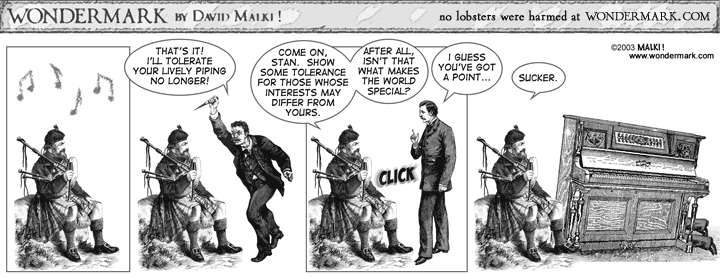
\includegraphics[width=0.9\textwidth]{bilder/comics/wondermark003.png}
% \end{figure*}

% TODO sind die Begriffe, die man für den Studienplan braucht, hier gut untergebracht oder sollten die mit in den restlichen Erklärungstext? Ist das hier wirklich eine kurze, neutrale Begriffserklärung oder nicht eher ein Kapitel "Kritische Kommentrare zu den Vorlesungen und Übungen"?

Einen guten überblick über die an der Uni gebräuchlichen Begriffe und
Abkürzungen findest du im "`Uni-ABC"' des AStA-Erstiinfos. Im folgenden
sind nur die wichtigen Begriffe für deinen Stundenplan erklärt, den du
auf der letzten Seite dieses Heftes findest.




% TODO Spätestens hier (Noch Fragen?) hört's auf, die Fragen sind keine Begriffsklärung mehr. Das ist ja gut, dass es solche Texte gibt, aber die Überschrift passt einfach nicht.
\subsubsection*{Noch Fragen?}

Die Qualität dieser drei Veranstaltungsarten ist in starkem Maße vom
jeweiligen Vortragenden abhängig. Während du unter Umständen die
Seminargruppen noch wechseln kannst, so ist das bei den erstgenannten
Veranstaltungen natürlich nicht möglich.

Du wirst sehr bald feststellen, dass es verschiedene Lerntypen gibt. Manche
deiner Kommilitonen werden kaum eine Vorlesung besuchen, sondern stattdessen die großen
und kleinen übungen verschlingen. Wieder andere lassen sich sowieso kaum im
Hörsaal blicken, sondern können am besten zu Hause oder in der Uni-Bibliothek
autodidaktisch lernen.

Wenn trotz Vorlesungen, großer übungen und kleiner übungen noch Fragen
auftreten, so hilft dir das Gespräch mit den Kommilitonen oder der Blick in
entsprechende Literatur.
Wichtig: Kaufe nicht gleich jedes empfohlene Buch neu,
das ist Geldverschwendung. Frage höhere Semester nach wirklich sinnvoller
Literatur, leih' dir die Bücher aus der UB aus, gebrauchte Bücher gibt es
günstig z.B. in der Newsgroup \url{http://groups.google.de/group/braunschweig.kaufrausch/} (siehe den Artikel
ab Seite \pageref{elekinf}). An der Uni wird man nicht umsorgt wie etwa in der
Schule oder in der betrieblichen Ausbildung, du trägst ein wesentlich höheres
Maß an Eigenverantwortung. Zur Orientierung in der ersten Zeit ist ein
Ansprechpartner unentbehrlich. Wenn die Kommilitonen aus
deinem eigenen Semester nicht weiterhelfen können, dann vielleicht dein/e TutorIn oder andere
Studierende im höheren Semester (zum Beispiel Mitbewohner, Fachgruppe).
